
%(BEGIN_QUESTION)
% Copyright 2006, Tony R. Kuphaldt, released under the Creative Commons Attribution License (v 1.0)
% This means you may do almost anything with this work of mine, so long as you give me proper credit

It is possible to measure the level of a liquid-liquid interface by means of a float:

$$\includegraphics[width=15.5cm]{i00312x01.eps}$$

Explain what characteristic(s) the float must have in order to successfully hover at the interface level.  Also, describe some potential advantages this technique enjoys over interface methods based on hydrostatic pressure. 

\vskip 20pt \vbox{\hrule \hbox{\strut \vrule{} {\bf Suggestions for Socratic discussion} \vrule} \hrule}

\begin{itemize}
\item{} Identify some practical applications of liquid interface level measurement in industry.
\item{} Suppose an instrument technician replaced the ``tape'' in this level instrument, and accidently substituted one that was 1.5 feet shorter than the old tape.  Assuming all else in this instrument remained the same, how would its calibration be affected?  Would we see a zero shift, a span shift, a change in linearity, or some combination of these?
\end{itemize}

\underbar{file i00312}
%(END_QUESTION)





%(BEGIN_ANSWER)


%(END_ANSWER)





%(BEGIN_NOTES)

There is one main float criterion that must be met:

$$D_{fluid(light)} < D_{float} < D_{fluid(heavy)}$$

\vskip 10pt

Potential advantages of float measurement over hydrostatic measurement:

\begin{itemize}
\item{} Immunity from slight changes in fluid densities
\item{} No need for a fixed fluid height (overflow at top of vessel)
\end{itemize}

\vskip 10pt

We could make a custom float out of hollow metal, then fill that hollow metal container with some heavy substance (liquid or solid) until its overall ``density'' was just right. 

%INDEX% Measurement, interface level: float

%(END_NOTES)


